\documentclass[./examen.tex]{subfiles}

\begin{document}

\info{Evaluación Electrotécnia II}{f.e.m generada por un conductor que se mueve en un campo magnético.}
\begin{center}
\makebox[\textwidth]{Nombre y Apellido:\enspace\hrulefill}
\end{center}
\begin{questions}

 \question[5] Un conductor que se desplaza con una velocidad $v=300\frac{m}{s}$ perpendicular a un campo magnético de inducción $B=11.1T$, sabiendo que la longitud es $l=20cm$. Calcular la fuerza electro motriz $f.e.m$ inducida en el conductor en volts $V$.
 
 \begin{center}
 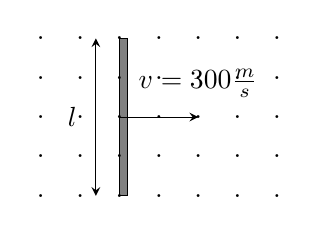
\begin{tikzpicture}
 \draw [stealth-stealth](-0.3,0) -- (-0.3,2);
 \node at (-0.6,1) {$l$};
 \draw [fill=gray](0,0) rectangle (0.1,2);
 \draw [-stealth] (0,1) -- (1,1)  node[label={$v=300\frac{m}{s}$}]{};
 \foreach \y in {0,1,2,...,4}{
    \foreach \x in {-2,-1,0,...,4}{
    \node at (\x/2,\y/2) {.};
    }
}
 \end{tikzpicture}
 \end{center}
 
 \question[5]  Una bobina de $N=400$ espiras es recorrida por una corriente $I=20A$ que da lugar a un flujo magnético de $\Phi=0,001Wb$. Calcular el coeficiente de autoinducción $L$ de la bobina.
 \end{questions}

 
 \end{document}